% THIS IS AN EXAMPLE DOCUMENT FOR VLDB 2012
% based on ACM SIGPROC-SP.TEX VERSION 2.7
% Modified by  Gerald Weber <gerald@cs.auckland.ac.nz>
% Removed the requirement to include *bbl file in here. (AhmetSacan, Sep2012)
% Fixed the equation on page 3 to prevent line overflow. (AhmetSacan, Sep2012)

\documentclass{vldb}
\usepackage{graphicx}
\usepackage{mymacros}

\usepackage{balance}  % for  \balance command ON LAST PAGE  (only there!)


\begin{document}

% ****************** TITLE ****************************************

\title{Analysis of Multi-Join Benchmarking}

% possible, but not really needed or used for PVLDB:
%\subtitle{[Extended Abstract]
%\titlenote{A full version of this paper is available as\textit{Author's Guide to Preparing ACM SIG Proceedings Using \LaTeX$2_\epsilon$\ and BibTeX} at \texttt{www.acm.org/eaddress.htm}}}

% ****************** AUTHORS **************************************

% You need the command \numberofauthors to handle the 'placement
% and alignment' of the authors beneath the title.
%
% For aesthetic reasons, we recommend 'three authors at a time'
% i.e. three 'name/affiliation blocks' be placed beneath the title.
%
% NOTE: You are NOT restricted in how many 'rows' of
% "name/affiliations" may appear. We just ask that you restrict
% the number of 'columns' to three.
%
% Because of the available 'opening page real-estate'
% we ask you to refrain from putting more than six authors
% (two rows with three columns) beneath the article title.
% More than six makes the first-page appear very cluttered indeed.
%
% Use the \alignauthor commands to handle the names
% and affiliations for an 'aesthetic maximum' of six authors.
% Add names, affiliations, addresses for
% the seventh etc. author(s) as the argument for the
% \additionalauthors command.
% These 'additional authors' will be output/set for you
% without further effort on your part as the last section in
% the body of your article BEFORE References or any Appendices.

\numberofauthors{2} %  in this sample file, there are a *total*
% of EIGHT authors. SIX appear on the 'first-page' (for formatting
% reasons) and the remaining two appear in the \additionalauthors section.

\author{
% You can go ahead and credit any number of authors here,
% e.g. one 'row of three' or two rows (consisting of one row of three
% and a second row of one, two or three).
%
% The command \alignauthor (no curly braces needed) should
% precede each author name, affiliation/snail-mail address and
% e-mail address. Additionally, tag each line of
% affiliation/address with \affaddr, and tag the
% e-mail address with \email.
%
% 1st. author
\alignauthor
Harshad Deshmukh\\
       \affaddr{University of Wisconsin-Madison}\\
       \email{harshad@cs.wisc.edu}
% 2nd. author
\alignauthor
Jignesh M. Patel\\
       \affaddr{University of Wisconsin-Madison}\\
       \email{jignesh@cs.wisc.edu}
}

\maketitle

\begin{abstract}

\end{abstract}
\section{Introduction}
Performance of join operations is crucial for relational data analytics. 
For a long time, database community has tried to improve the performance of join operations. 
The two main approaches in join algorithm designs are - partition-based and no partition-based join implementations. 

Remarkably, most of the prior work on join performance~\cite{DBLP:conf/sigmod/BlanasLP11,DBLP:conf/sigmod/SchuhCD16} has focused on a single join, usually implemented with synthetic schema and data. 
The prior work is valuable in understanding the implications of various parameters on the performance of one join operation. 
However, real life decision support queries often involve multiple join operations (multi-join), typically executed one after another on a dataset organized as star-schema or snowflake-schema. 
The debate on partitioning-based \textit{vs} no partitioning-based joins has not been extended to the settings of multi-joins. 

An additional complexity associated with analyzing multi-joins is the potential re-partitioning operation between two joins. 
The re-partitioning is needed when the input to the partitioned join is either not partitioned at all or is partitioned on a different attribute than the join attribute.

Our goal is to devise a high performance hash-based multi-join implementation algorithm for a right deep pipeline.
\reminder{Justify why we choose only hash-based implementations}.
One example of a right deep pipeline is shown in Figure~\ref{fig:right-deep-pipeline}.

\begin{figure}[t]
	\centering
	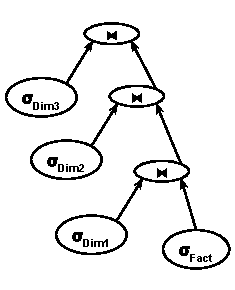
\includegraphics[]{figures/right-deep-pipeline.pdf}
		\vspace*{-1.5em}
	\caption{\textbf{A right-deep pipeline consisting of three join operations. $Dim_i$ indicates $i^{th}$ dimension table and $Fact$ denotes the fact table in a star-schema.}}
	\label{fig:right-deep-pipeline}
		\vspace*{-1.5em}
\end{figure}

An important aspect of the right-deep pipeline in Figure~\ref{fig:right-deep-pipeline} is that the build side in all the join operations is always some dimension table. 
We will leverage this aspect of the right-deep pipeline in our algorithm design. 
\reminder{Think of extending the idea to left-deep or zig-zag trees.}

Also note that Figure~\ref{fig:right-deep-pipeline} is a \textit{logical plan} produced by the optimizer. 
It gives information about join ordering. e.g. join between $Fact$ and $Dim_1$ relations should be performed first, followed by the join of the first join's result and $Dim_2$ relation. 
Figure~\ref{fig:right-deep-pipeline} does not specify the type of join (e.g. hash-based or sort-merge) and/or the partitioning nature of the join such as radix-based partitioned join or no partition-based join. 

The goal of our algorithm is to produce a high performance \textit{physical plan} which consists of the partitioning nature of each join in the pipeline.
We formally describe the problem in the next section.

\subsection{Problem Statement}
Given a right deep pipeline (as shown in Figure~\ref{fig:right-deep-pipeline}), consisting of $k$ join operations viz. $J_1, J_2, \ldots J_k$, between fact and dimension tables, find the partitioning characteristic of the implementation of each join $p(J_i)$, which can result in overall high performance of the pipeline. 

Our objective is to minimize the execution time of the multi-join pipeline. 
Let us define the execution time of join operation (probe + build phase) $J_i$ as $T(J_i)$, or simply $T_i$. 
Therefore the objective is to minimize $\sum\limits_{i=1}^{k}T_i$.

Note than if the execution exhibits pipelined parallelism, the above objective might be incorrect. 
In such a case, the total execution time for the pipeline is simply the time difference between end of execution of the last join and beginning of execution of the first join. 

We consider only two options for the partitioning characteristic of the join implementation, i.e. $p(J_i) := \textsc{partition-based}$ or $p(J_i) := \textsc{No partition-based}$. 
Thus, our problem can be viewed as an assignment problem, where we have to assign a value to $k$ binary variables.
Therefore, the size of the solution space is $2^k$, i.e. there are $2^k$ number of different possible physical plans. 

In the next section, we discuss some proposals to solve the above problem. 

\subsection{Proposed Methodology}
We first discuss the parameters involved in this problem. 
The execution time $T_i$ per join operation $J_i$ consists of both build and probe phases.
If the join implementation is partitioning-based, then the time to partition (or re-partition)the relations is included in $T_i$.

We use a metric to differentiate the performances of partitioned and non-partitioned probes. 
This metric is the number of CPU cycles per probing tuple ($C_{probe}$), and it is impacted by the size of the probed hash table $Size_{HT}$. 
In the two implementations, viz. partitioned and non-partitioned the relationship between $C_{probe}$ and $Size_{HT}$ is different. 
We study this relationship and estimate the cost of a given probe operation. 
In the next section, we present some initial empirical results to understand this relationship.

The partitioned implementation of a join operator may consist of partitioning cost. 
Therefore, we define another metric $C_{part}$, which is the number of CPU cycles spent in partitioning a single input tuple. 

Finally, we estimate the cost of each join operations in terms of CPU cycles per input tuple. 

We may use a well known technique such as dynamic programming to solve the assignment problem. 

Note that we restrict ourselves to one form of materialization of the results i.e. eager materialization. 
This means that each join operation's result is immediately materialized as soon as the operation is complete. 
(An alternative could be late materialization, as is used by MonetDB.)
\reminder{Unanswered question: Do assignment change as the query is in progress? e.g. If there are skewed results of the lower join operations in the query plan.}

\subsubsection{Heuristics}
As described earlier, the total number of possible physical plans is exponential in the number of join operations. 
It may be prohibitively expensive to analyze all possible plans. 
Therefore, we can prune the number of plans being analyzed, by applying some heuristics.
Examples of such heuristic could be: flip-flop between partitioned and non-partitioned joins is not desirable for successive join operations, prefer partitioned joins for lower level join operations in a query plan. 
\section{Experimental Evaluation}
Evaluation description goes here. 
\section{Conclusions}
Based on this preliminary analysis, we can draw some conclusions which are described below:%\footnote{Assuming that we trust the benchmark results.} 
\begin{enumerate}
	\item{Larger hash tables (size greater than the size of the L3 cache) are not desirable for probe performance.}
	\item{The CPU cycles per input tuple remains fairly stable for a large spectrum of hash table sizes i.e. Hash table sizes larger than L1 and smaller than L3. An implication of this observation could be that less efforts could be spent in tuning the partition size; as long as the partition size is within the range [L1, L3], the performance will be similar. }
	\item{Hyper threading adversely affects the probe performance, however the impact is higher for larger hash tables (size greater than 2*L3)}
\end{enumerate}

\section{Related Work}
The database community has paid significant attention to improve join performance in the past decade. 
Blanas et al.~\cite{DBLP:conf/sigmod/BlanasLP11} analyzed the join performance in single socket, large main-memory server environments using various join implementations such as radix-based partitioning, no-partitioned join and using uniform as well as skewed data sets. 

Schuh et al.~\cite{DBLP:conf/sigmod/SchuhCD16} reviewed various join implementations from the research literature from the past decade. 
They classified the join algorithms in two categories - partitioning based and no-partitioning based join algorithms, and compared their performance characteristics. 
As they observed, prior work on join performance has mostly focused on synthetic queries and synthetic datasets. 
In the interest of discussing the join algorithm performance in the context of real life queries, they measured the performance of various join algorithms on a real query (TPC-H Query 19). 

% ensure same length columns on last page (might need two sub-sequent latex runs)
\balance

% The following two commands are all you need in the
% initial runs of your .tex file to
% produce the bibliography for the citations in your paper.
\bibliographystyle{abbrv}
\bibliography{refs}  % vldb_sample.bib is the name of the Bibliography in this case
% You must have a proper ".bib" file
%  and remember to run:
% latex bibtex latex latex
% to resolve all references

%APPENDIX is optional.
% ****************** APPENDIX **************************************
% Example of an appendix; typically would start on a new page
%pagebreak

\end{document}